\section{Einleitung}
Im vorliegenden Bericht werden die Ergebnisse des Projekts "Berlin Mobility - Verkehrsanalyse im Raum Berlin" aufbereitet und vorgestellt. Das Projekt wurde vom Oktober 2020 bis Februar 2021 unter Federführung der Berliner Senatsverwaltung für Umwelt, Verkehr und Klimaschutz durchgeführt. Die Senatrsverwaltung wurde bei der Projektdurchführung und der wissenschaftlichen Ausgestaltung des Vorhabens durch Experten des Fachbereichs Big Data \& Business Analytics der FOM-Hochschule für Wirtschaft und Oekonomie unterstützt. 


\subsection{Problemstellung}
Mobilität befindet sich im ständigen Wandel. Das trifft insbesondere auf urbane Mobilität in Metropolen wie London, Tokyo und Berlin zu, was auf zwei Faktoren der fortschreitenden Urbanisierung zurückzuführen ist. Aufgrund des kontinuierlichen Zuzugs ist die Einwohnerzahl Berlins in den letzten \todo[inline]{XX Jahren um XX \% gestiegen.} Gleichzeitig nimmt die Stadtfläche kontinuierlich zu. Allein zwischen 1991 und 2010 ist Berlin in der Fläche um \todo[inline]{xx \% gewachsen.} \todo[inline]{Quelle Flächenentwicklung Berlin PDF.} Beide Entwicklungen stellen für die Planung und Gestaltung einer zukunftssicheren Verkehrsinfrastruktur große Herausforderungen dar. Eine entsprechende Verkehrsplanung muss sicherstellen, dass die Mobilität heute reibungslos funktioniert und zukünftigen Mobilitätsansprüchen auf einer größeren Fläche und mit steigenden Fahrgastzahlen genügt. 

Im Juni 2018 hat das Berliner Abgeordnetenhaus zu diesem Zweck ein neues Mobilitätsgesetz beschlossen. Ziel des Berliner Mobilitätsgesetzes ist es, eine belastbare Grundlage zur Gestaltung einer zukunftsfähigen urbanen Mobilität für die Hauptstadt zu schaffen. Berlin soll mobiler, sicherer und klimafreundlicher werden. Dafür sollen Stärken aller zur Verfügung stehenden Verkehrsmittel genutzt werden. Der ÖPNV soll stark ausgebaut werden und unterschiedliche Verkehrsmittel stärker miteinander vernetzt werden. Zudem soll die Fahrradinfrastruktur deutlich verbessert werden. Durch die Summe der Maßnahmen soll die Leistungsfähigkeit des Verkehrssystems gesteigert und die Lebensqualität der Berliner erhöht werden. Das Ziel des Mobilitätsgesetzes ist es, eine Verkehrswende einzuläuten und den PKW-Verkehr bis 2050 klimaneutral zu gestalten. 

Die Umsetzung des Berliner Mobilitätsgesetztes ist wegweisend für die Berliner Mobilität der Zukunft. Investitionen die ausgehend von dem im Mobiltiätsgesetz beschriebenen Maßnahmen getätigt werden, werden die Verkehrsinfrastruktur und die Mobiltität in der Stadt langfrsitig prägen. Es ist also von zentraler Bedeutung, sicherzustellen, dass an den richtigen Stellen investiert wird und die Umsetzung effizient vorangetrieben wird. 

 Bereits in den ersten zwei Jahren nach Beschlussfassung, sind die Planung und Umsetzung des Berliner Mobilitätsgesetztes regelmäßig Ziel öffentlicher Kritik. Dabei wird beanstandet, dass Maßnahmen unzureichend geplant seien und die Umsetzung nur schleppend vorangehe. \todo[inline]{Probleme hier näher beschreiben und quellen einfügen.} Zudem herrscht zwischen den agierenden politischen Akteuren weiterhin Uneinigkeit über den Stellenwert, der dem Autoverkehr zukünftig zugeschrieben werden soll.

\subsection{Zielsetzung}
Mit dem Projekt "Berlin Mobility - Verkehrsanalyse im Raum Berlin" verfolgt die Berliner Senatrsverwaltung für Umwelt, Verkehr und Klimaschutz das Ziel Daten für die Verkehrsanalyse sowie die Verkehrsgestaltung in der Stadt Berlin nutzbar zu machen. Daraus leiten sich zwei Kernziele ab. Zunächst soll ausghend von einschlägigen Mobilitätsdaten, Geodaten und Populationsdaten Zukm einen 

\subsection{Aufbau der Arbeit}
Kapitel \ref{infos} enthält die Inhalte des Thesis-Days und alles, was zum inhaltlichen erstellen der Thesis relevant sein könnte. In Kapitel \ref{latexDetails} \nameref{latexDetails} findet ihr wichtige Anmerkungen zu \LaTeX{}, wobei die wirklich wichtigen Dinge im Quelltext dieses Dokumentes stehen (siehe auch die Verzeichnisstruktur in Abbildung \ref{fig:verzeichnisStruktur}).


\begin{figure}[H]
\caption{Verzeichnisstruktur der \LaTeX{}-Datein}\label{fig:verzeichnisStruktur}
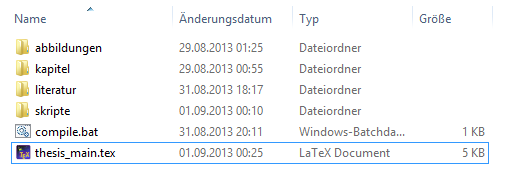
\includegraphics[width=0.9\textwidth]{verzeichnisStruktur}
\\
Quelle: Eigene Darstellung
\end{figure}
